\documentclass[handout]{beamer}
\usepackage[frenchb]{babel}
\usepackage[T1]{fontenc}
\usepackage[utf8]{inputenc}
\usepackage{epstopdf}
% functions to plot
\def\func(#1){(#1)*(1-(#1))}
\hypersetup{colorlinks = true,linkcolor = blue,urlcolor  = blue}

\newcommand{\qGraph}[1]{\begin{center} \includegraphics[width =
\textwidth]{#1}\end{center}}

\newcommand{\mcl}{\mathcal}


\newenvironment{iPar}[1]{\textbf{#1} \begin{itemize}}{\end{itemize}}

\newcommand{\inc}{{inc}}
\newcommand{\cp}{{cmp}}
\newcommand{\bull}{$\bullet\;$} 

\newcommand{\esp}{\mathbf{E}} \newcommand{\ul}[1]{\underline{#1}}
\newcommand{\ol}[1]{\overline{#1}} \newcommand{\ora}[1]{\textbf{#1}}

\newcommand{\mdp}{\medskip \pause}

\title{Measuring Welfare and Well-Being}
\author{Microeconomics \\ 20851}
\date{}

\begin{document}

\frame{\titlepage}

\section[Outline]{}
\frame{\tableofcontents}

\section{}

\section{Utilitarian approach}

\begin{frame}\frametitle{Measuring Well-Being}

\textbf{Naive utilitarian approach}

\begin{itemize} \item For each citizen $i
\in \{1,\ldots,N\}$, find the utility function $U_i$ which represents his/her preferences on the baskets found in $B$
\item Suppose that the citizens obtain the baskets $B_1$, $B_2$, ..., $B_N$

\item Well-being: $U_1(B_1) + U_2(B_2) + \ldots + U_N(B_N)$
\item A policy $\mcl P_0$ is better than an alternative $\mcl P_1$ if it provides more well-being.
\end{itemize}
\end{frame}
 

\begin{frame}\frametitle{Why Naive Utilitarianism is Inadequate}
\textbf{Preferences are ordinal} \begin{itemize}\item If $U_1$ represents the preferences of citizen $1$, $f(U_1)$ represents the same preferences for any strictly increasing function $f$ \item For example, we could have used $2
\times U_1$. \end{itemize}\mdp

\textbf{The implications are not well defined} \begin{itemize} \item  $\mcl P_0$ better if $WF = U_1 + U_2$
\item $\mcl P_1$ better if $WF = 2U_1 + U_2$ \item Well-being should only depend on preferences and not on $U$. \end{itemize}

\end{frame}

\section{Compensating variations}

\begin{frame} \frametitle{Define Well-Being by Preferences}
\textbf{Indirect Utility} \begin{itemize}
\item
Policy $\mcl P$ defines a budget constraint $C_i(\mcl P,I_i)$ for citizen $i$ (where $I_i$ is income)
\item The maximum utility of citizen $i$ given his constraint is: $$U_i^*(\mcl P,I_i) = \max_{B \in C_i(\mcl P, I_i)} U_i(B)$$
\item Example: two goods $X$ and $Y$. Utility $U(X,Y) = \ln X + \ln Y$ \medskip

Policy $\mcl P$: multiplicative tax $\tau$ on the price of
$Y$\mdp

$U_i^*(\mcl P,I) = \max_{X,Y} \ln X + \ln Y$ \\ s.c. $\quad \quad \quad
p_X  X + p_Y(1 + \tau) Y = I$ \end{itemize}
\end{frame}

\begin{frame}{Compensating Variation}
  \begin{itemize} \item Policy $\mcl P_0$ is the status
quo, implementing the new policy $\mcl P$ \item Compensating variation :  amount $\Delta I^{CV}$  such that $$U^*(\mcl P_0,I) = U^*(\mcl P,
I - \Delta I^{CV})$$    \item    Amount that we can take from the consumer while keeping his utility at the reference level (status quo).  

\item Note: sign convention is that  $\Delta I^{CV}>0$ when the policy change is \textit{good} 

 \end{itemize}
 
 \textbf{Exercise A}: Find the expression of the compensating variation for $\ln X + \ln Y$ and a tax $\tau$ on the good $Y$. 
\end{frame}

\begin{frame} \frametitle{Fundamental Property}

\textbf{The compensating variation only depends on preferences:} \begin{itemize} \item $\Delta I^{CV}$ only depends on preferences $$U^*(\mcl P_0,I) = U^*(\mcl P, I - \Delta I^{CV})
\Rightarrow 2 U^*(\mcl P_0,I) = 2  U^*(\mcl P, I- \Delta I^{CV})$$ \item Generally, for any function $f$, $$U^*(\mcl P_0,I) = U^*(\mcl P, I - \Delta I^{CV})
\Rightarrow f[U^*(\mcl P_0,I)] = f[ U^*(\mcl P, I - \Delta I^{CV})]$$\end{itemize}
 
\end{frame}
 
\begin{frame} \frametitle{Important Special Case}
\textbf{Quasi-linear utility} \begin{itemize} \item Preference for a good $X$ and money $Y$.
\item Preferences represented by
 $U(X,Y) = V(X) + Y$
\item Reference policy $\mcl P_0$: allocation $(X_0, Y_0)$
\item Change $\mcl P$: $(X_1, Y_1)$. \end{itemize} \mdp

\end{frame}

\begin{frame} \frametitle{Compensating Variation}

$\Delta I^{CV}$ such that
\begin{eqnarray*}
U(X_0,Y_0) &=& U(X_1, Y_1- \Delta I^{CV}) \\
V(X_0) + Y_0 &=& V(X_1) + Y_1 - \Delta I^{CV} \\
\Delta I^{CV} &=& V(X_1) + Y_1 - V(X_0) - Y_0 \\
\Delta I^{CV} &=& U(X_1,Y_1) - U(X_0,Y_0)
\end{eqnarray*}

The compensating variation is equal to the change in utility 
 \end{frame}

\section{Consumer surplus}

\begin{frame} \frametitle{Consumer Surplus for purchases}

\textbf{Suppose that utility is quasi-linear} \begin{itemize} \item Good $X$
and money $M$. $U(X,M) = V(X) + Y$ \item Suppose $V$ concave ($dV/dX$
decreasing in $X$) 
\item Consider   $\mcl P_0$ can't buy $X$  
\item Alternative $\mcl P$ allows the purchase of $X$ at price $p_X$ \\\mdp
$\max_{X,Y} U(X,Y) \quad s.t. \quad p_X X + Y = I$

\item Equivalent to $\max_{X} V(X) + I - p_X X$
\\ FOC: $ \frac{dV}{dX}_{|X^*} =  p_X$\\ Gives the demand $X^*(p_X)$ \end{itemize}\mdp

\end{frame}

\begin{frame}{Consumer Surplus}

Compensating variation from $\mcl P_0$ to $\mcl P$ is the consumer surplus. 

\begin{eqnarray*}
\Delta I^{CV} &=& V[X^*(p)] + I - pX^*(p) - [V(0) + I] \\
&=& V[X^*(p)] - V(0) - p X^*(p)
\end{eqnarray*}

\end{frame}

\begin{frame} \frametitle{Loss of Well-Being Generated by a Tax}
\textbf{Tax: going from $p_X = p+t$    to $p_X = p$  .} \begin{itemize}
\item New consumption $X^*(p) > X^*(p+t)$ \item Tax revenue $T
= t\times X^*(p+t)$ \item Compensating variation 
\begin{eqnarray*}
U[X^*(p), I - pX^*(p)] - U[X^*(p+t), I - (p+t) X^*(p+t)]
\end{eqnarray*}
\end{itemize}\mdp


\textbf{Property} \begin{itemize} \item $\Delta I^{CV} > T$: how much the consumer is willing to pay to avoid a tax higher than the revenue generated by the government \item Loss of well-being associated to the tax $= \Delta I^{CV} - T$ \end{itemize}



\end{frame}

\begin{frame} \frametitle{Loss of Well-Being Generated by a Tax}

\textbf{Exercise B}: If $V(X) = 10 X - \frac{1}{2}X^2$, find the loss of well-being generated by a tax $t$ on the good $X$. 
\end{frame}

\section{Application: Value of clean air}
\begin{frame}{Application: Value of clean air }
\begin{iPar}{A political question}
\item There is no market for clean air, it has to be protected (offered) by the government.
\item The Clean Air Act (1977): U.S. government put in place measures to reduce pollution.
\item E.g. 1990: Controlling vehicle emissions
\item Laws are costly to implement, paid indirectly by taxes which lead to higher prices
\item Question: do these measures increase well-being?
\end{iPar}\mdp

\begin{iPar}{How to answer this question}
\item Consider a change from policy $\mcl P_0$: no control, no costs, to $\mcl P$: pollution control which comes at a price
\item Compensating variation >0 (sign convention), citizens value this policy.
\end{iPar}
\end{frame}


\begin{frame}{How can we do it?}
\begin{iPar}{Step 1: Estimate people's preferences}
\item Find a situation where people have to balance pollution and wealth (consumption).
\item E.g. Buying a house. Very variable within a city.\mdp
\item \textbf{Controlling for other factors}, use data from real estate transactions to determine the value given to clean air
\item e.g. Define X = measure of clean air \\ (e.g. concentration of particles) \pause

Estimate using econometrics $U(X, Y) = V(X) + Y = \alpha X + \beta X^2 +Y$

\end{iPar}\mdp 

\end{frame}

\begin{frame}{Evaluating a Policy}

\begin{iPar}{Calculating a compensating variation}
\item Government spends $X_{GOV}$. This comes at a cost $c\times X_{GOV}$ for taxpayers (use the loss of well -being per dollar of tax revenue).
\item Consider a change from policy   $(0,0)$ to  $(X_{GOV}, - c \times X_{GOV})$
\item The consumer surplus is the compensating variation $\Delta I^{CV} =  V(X_{GOV}) - c X_{GOV} - V(0)$.
\end{iPar}\mdp

\begin{iPar}{Optimal pollution}
\item The optimal pollution value is the one which maximizes $U(X) = V(X) + I - c X$  \mdp
the FOC is
$$\frac{dV}{d X}_{|X^*} = c$$
\end{iPar}

\end{frame}



\begin{frame}{Evaluating the Value Given to Clean Air}
\begin{figure}
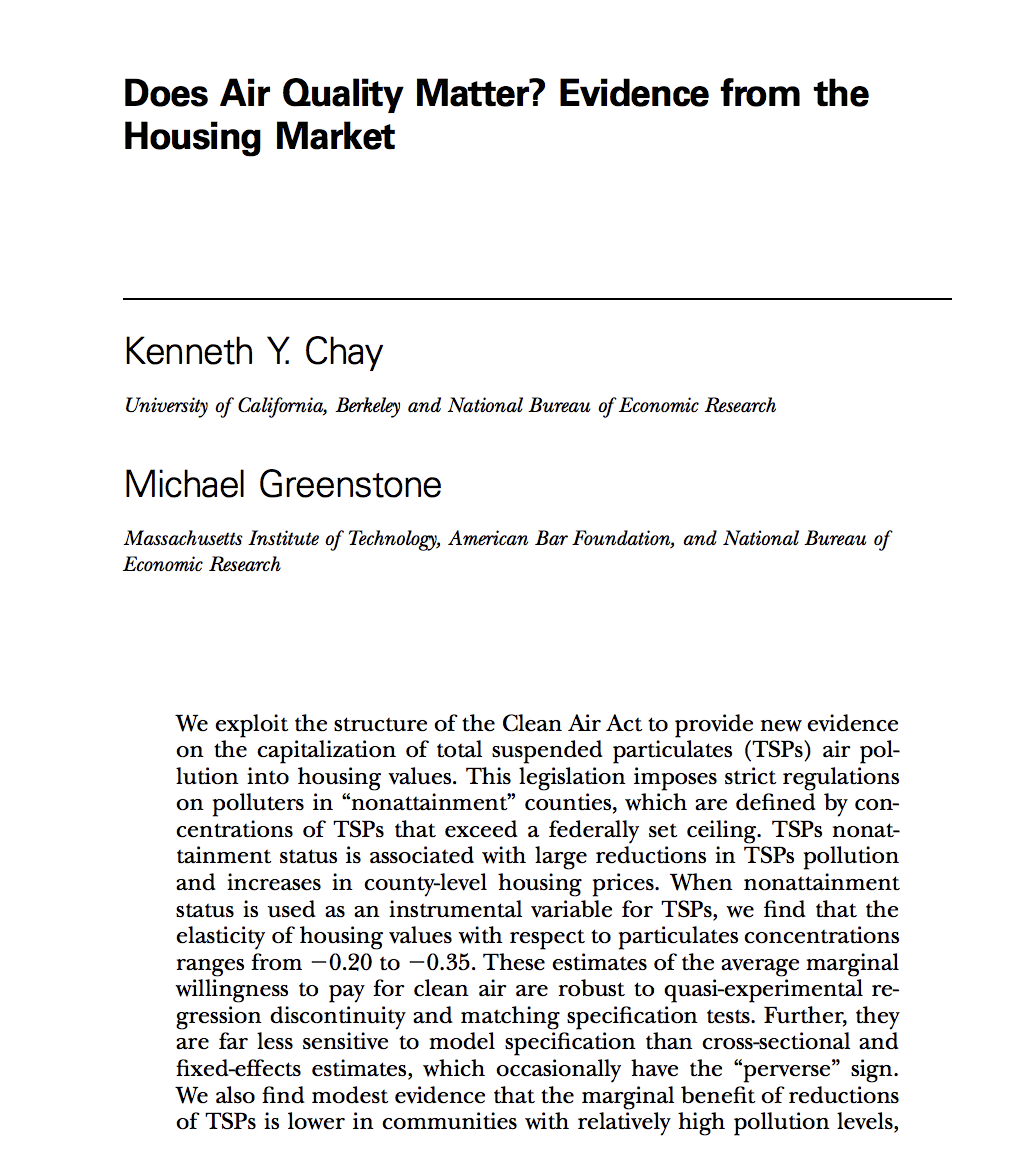
\includegraphics[scale=0.3]{chay.png}
\caption{\href{https://www.jstor.org/stable/10.1086/427462}{Chay et Greenstone (2005), Journal of Political Economy}}
\end{figure}
\end{frame}

\begin{frame}{Example: Noise Pollution}

\begin{itemize}
	\item The price elasticity of houses to noise pollution is -0.2
	\item The government is considering reducing the noise pollution on the side of a highway by 10\% .
	\item The engineers tell us that building the noise-cancelling wall will cost 1000\$ per affected homeowner
	\item This policy is financed by a tax which leads to a loss of well-being equivalent to 43 cents for every tax dollar. 
\end{itemize}
	
\textbf{Exercise C}: Does this policy increase the well-being of the affected homeowners?
\end{frame}

\section{Measuring happiness}

\begin{frame}{Directly measuring well-being}

\begin{itemize}
\item The compensating variation approach is due to \href{https://fr.wikipedia.org/wiki/John_Hicks}{John Hicks}
\item Why not just ask people whether they are happy?
\item New-Zealand project
\item \href{https://fr.wikipedia.org/wiki/Richard_Easterlin}{Richard Easterlin} popularized this ( the relation between happiness and income per head is almost zero)
\end{itemize}


\end{frame}

\begin{frame}{The Easterlin Paradox}

\begin{figure}
\centering
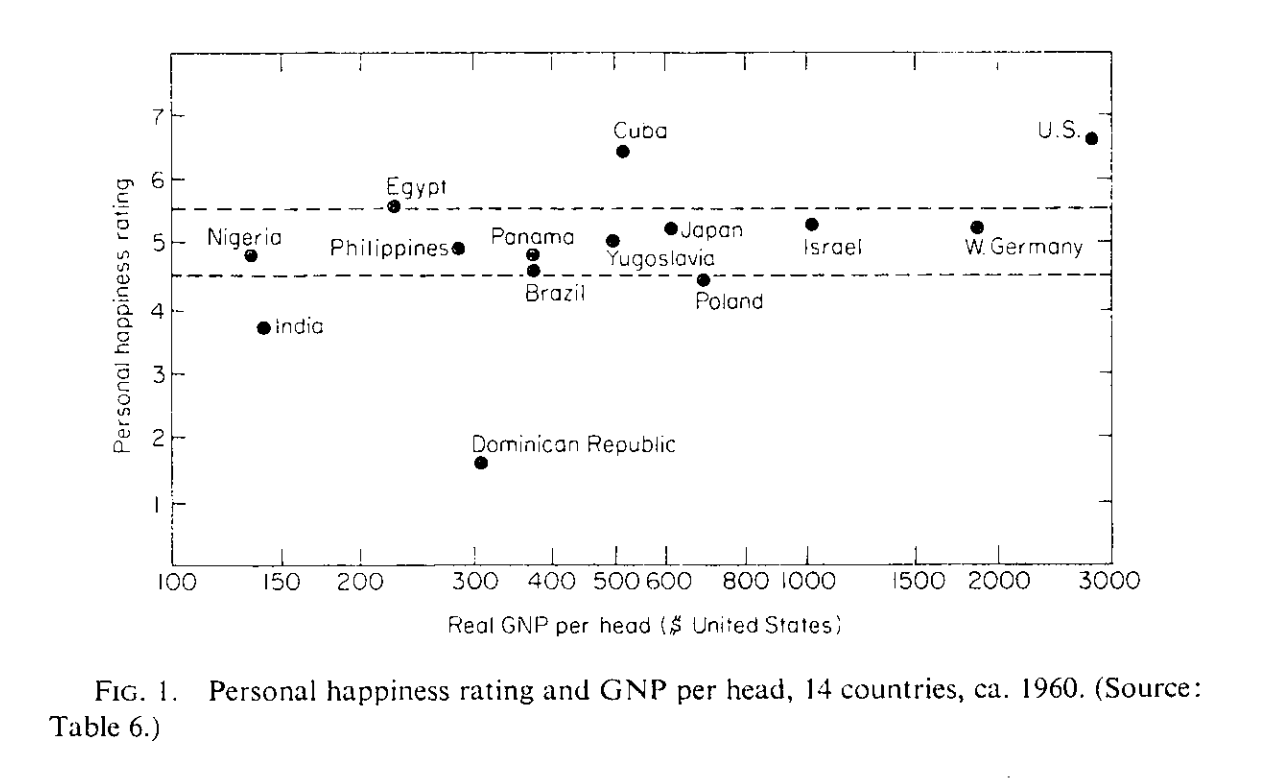
\includegraphics[scale=0.3]{easterlin.png}
\caption{\href{http://graphics8.nytimes.com/images/2008/04/16/business/Easterlin1974.pdf}{Easterlin (1974)}}
\end{figure}

\end{frame}


\begin{frame}{Is there a paradox?}

\begin{figure}
\centering
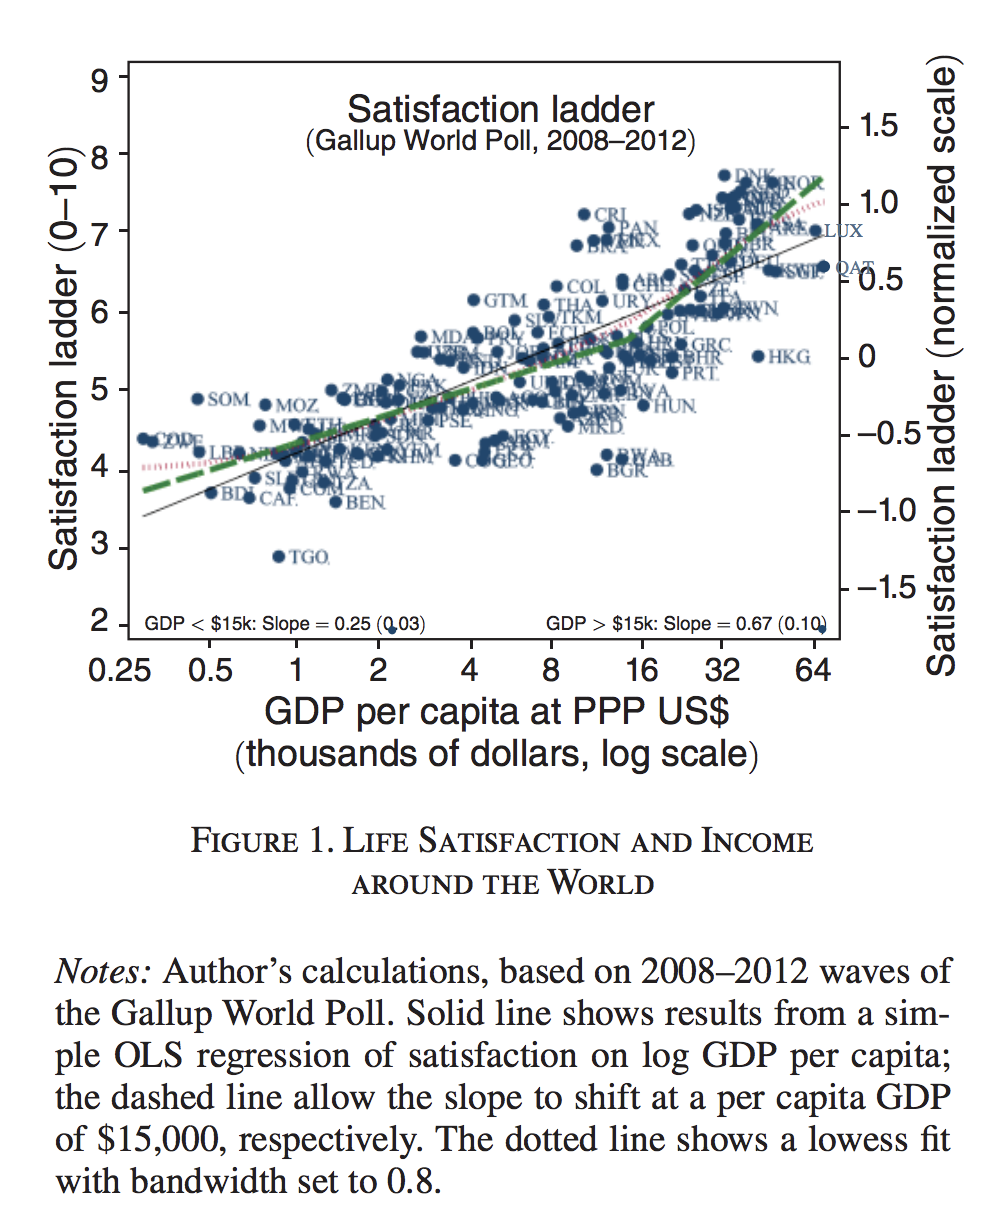
\includegraphics[scale=0.3]{wolfers.png}
\caption{\href{http://users.nber.org/~jwolfers/papers/Satiation(AER).pdf}{Stevenson and Wolfers (2013), AER: Papers and Proceedings}
}
\end{figure}

\end{frame}

\begin{frame}{Using Well-Being Measures to Evaluate a Policy}

\begin{itemize}
\item Why not look at a policy's impact on happiness?
\item Pros: a direct evaluation without a model takes all dimensions into account
\item Cons: people have different ways of measuring happiness, choosing the right question is difficult, many psychological effects at play
\end{itemize}

We see very few studies include these measures in policy evaluation. However, we also see a lot of interest from governments. 
\end{frame}

\end{document}




